% !TeX root = main.tex

\section{Analyse du métier, de la donnée et des enjeux documentaires}
\label{sec:analyse_metier}

À la suite de la présentation des objectifs du projet (Chapitre~1), ce chapitre approfondit les contraintes propres à la situation du projet, justifiant les choix effectués par la suite car dépendant du lieu d'activité. Il précise la distinction entre le cadastre et les actes, explique le fonctionnement du versement sur Géofoncier via son API REST, caractérise les différents types d'archives, puis évoque la problématique de la filiation parcellaire. Enfin, il synthétise les contraintes de confidentialité et d'exécution locale.

\subsection{Cadastre et propriété foncière : distinction juridique}

Pour comprendre l'intérêt des archives, il est important de faire la différence entre le plan cadastral et les actes de bornage, l'interêt étant différent.

Créé en 1807 sous le régime de Napoléon I\textsuperscript{er}, le cadastre français avait à l'origine un objectif uniquement fiscal : recenser la totalité des propriétés foncières afin de récolter de façon équitable l'impôt foncier. Aujourd'hui, le Plan Cadastral Informatisé (PCI), géré et mis à jour par la Direction Générale des Finances Publiques (DGFiP), sert de fond de plan de référence pour l'aménagement du territoire.

Cependant, en droit français, le cadastre ne constitue ni un titre de propriété ni une délimitation juridique des terrains. La jurisprudence de la Cour de cassation rappelle que le cadastre ne fournit qu'une présomption fiscale et parcellaire. De plus, la précision du PCI est très variable : dans les zones rurales issues d'anciens plans napoléoniens vectorisés, les écarts de positionnement des limites cadastrales par rapport au terrain réel peuvent dépasser plusieurs mètres.


À l'inverse, la délimitation d'une propriété relève du monopole légal du géomètre-expert, réaffirmé par la loi n$^\circ$46-942 du 7 mai 1946 (\hyperref[ann:textes_loi]{voir Annexe~A -- [1]}). Conformément à l'article 646 du Code civil (\enquote{Tout propriétaire peut obliger son voisin au bornage de leurs propriétés contiguës}), la limite réelle entre deux terrains ne peut être fixée de manière définitive que par un PV de bornage. Rédigé par le géomètre-expert et signé par l'ensemble des propriétaires riverains, ce PV de bornage est un acte contradictoire ayant valeur juridique opposable aux tiers. Lors de cette opération, le géomètre matérialise les limites sur le terrain par des repères physiques (bornes OGE, clous d'arpentage) et les rattache au système officiel Lambert-93 avec une précision centimétrique.

Ainsi, alors que le cadastre ne propose qu'un découpage administratif et fiscal à valeur indicative, les archives conservées au sein des cabinets constituent la seule mémoire juridique de la propriété foncière.

Cette opposition entre le rôle fiscal du cadastre et le rôle juridique du géomètre-expert explique pourquoi la conservation des archives privées est importante pour les cabinets. Lorsqu'un litige survient entre des propriétaires riverains, les juges s'appuient en priorité sur les procès-verbaux de bornage et les plans d'arpentage anciens rédigés sur le terrain par le géomètre. Le plan cadastral n'est consulté qu'à titre subsidiaire. La disparition ou l'altération d'un dossier historique priverait le cabinet et les propriétaires des éléments de preuve nécessaires pour rétablir une limite de propriété.

\subsection{Le versement sur Géofoncier (API REST et Swagger)}

Les opérations foncières réalisées par les géomètres-experts font l'objet d'un versement sur le portail Géofoncier, créé par l'OGE en 2010. Ce versement répond à l'obligation de centraliser et de référencer toutes les interventions sur le territoire. Comme l'illustre la figure~\ref{fig:interface_geofoncier}, ce dernier affiche sous forme de pastilles la géolocalisation des opérations réalisées par l'ensemble de la profession (\hyperref[ann:textes_loi]{voir Annexe~A -- [4]}), ici pour une commune locale. Ce système permet aux cabinets de vérifier immédiatement si des travaux de bornage ou de division existent déjà sur une parcelle et de retrouver le géomètre qui a réalisé l'opération.

\begin{figure}[H]
  \centering
  \setlength{\fboxsep}{0pt}%
  \setlength{\fboxrule}{0.5pt}%
  \fbox{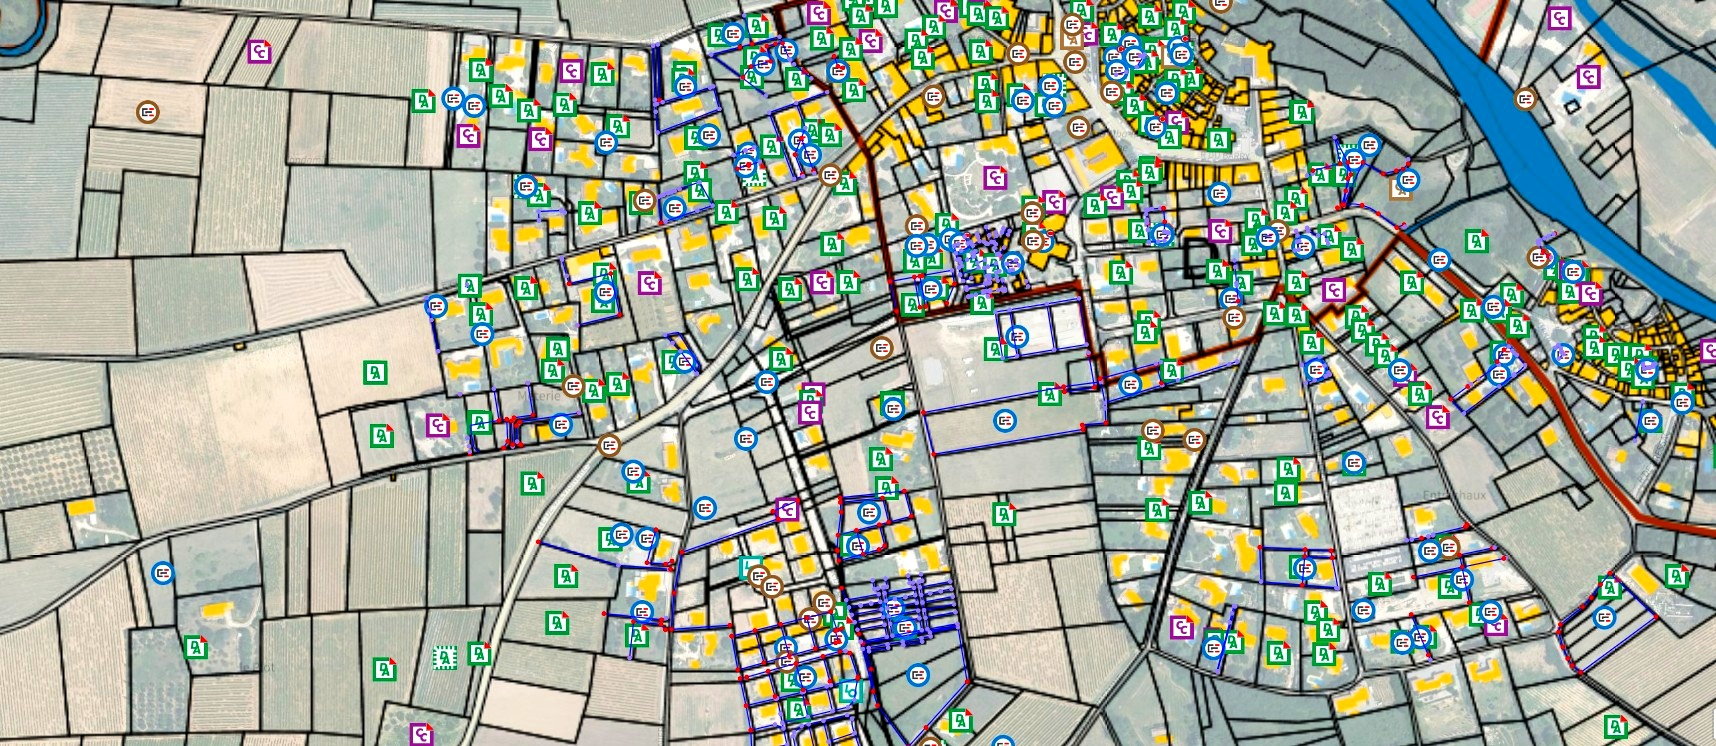
\includegraphics[width=0.85\textwidth]{img/Chap2_pastilles_enhanced.jpg}}\par
  \vspace{0.5em}
  \caption{Capture d'écran du portail GéofoncierEXPERT.}
  \label{fig:interface_geofoncier}
\end{figure}

Pour verser automatiquement des dossiers sans passer par une saisie manuelle sur le site web, l'OGE met à disposition une API REST (\hyperref[ann:textes_loi]{voir Annexe~A -- [5]}). L'ensemble des routes et des méthodes d'échange est documenté via une interface Swagger UI, qui permet de tester les requêtes et de consulter les formats attendus pour chaque composante (notamment `rfuoge` pour le RFU et `dossiersoge` pour la gestion des dossiers).

Le fonctionnement du versement repose sur plusieurs étapes. En principe, un serveur de préproduction est prévu pour tester les versements sans impacter la base réelle. Cependant, lors des travaux sur ce projet, le serveur de préproduction était indisponible et ne permettait pas de générer de jetons d'accès. Les développements et la constitution des requêtes ont donc été réalisés en s'appuyant directement sur les spécifications officielles de l'API.

L'accès aux services de l'API nécessite l'envoi d'un jeton d'authentification (Token) transmis dans l'en-tête HTTP de chaque requête, délivré après authentification des identifiants du géomètre-expert, et renouvelable toutes les 24 heures.

L'enregistrement d'une opération sur l'endpoint `rfuoge` nécessite de fournir une structure au format JSON contenant plusieurs informations obligatoires. Ces données comprennent le code INSEE à 5 chiffres de la commune (issu du Code Officiel Géographique \citep{insee_cog}), la date de l'acte au format ISO 8601 (`AAAA-MM-JJ`), le type d'acte selon le code OGE (par exemple `Bo` pour un bornage, `DA` pour un document d'arpentage), la référence interne du dossier au cabinet, ainsi que les coordonnées du centroïde ou l'emprise de l'opération en Lambert-93 (EPSG:2154). Un exemple de payload valide est présenté en figure~\ref{fig:payload_json_geofoncier}. L'objectif du projet est donc de concevoir une chaîne de traitement capable d'extraire automatiquement l'ensemble de ces éléments depuis les archives.



\begin{figure}[H]
  \centering

  \begin{verbatim}
  {
    "code_insee": "07019",
    "date_operation": "1984-05-12",
    "type_acte": "Bo",
    "reference_dossier": "GEO-1984-089",
    "geometry": {
      "type": "Point",
      "coordinates": [801452.35, 6391204.18]
    }
  \end{verbatim}
  \caption{Exemple de structure de données JSON transmise à l'API REST de Géofoncier pour enregistrer une opération (valeurs fictives).}
  \label{fig:payload_json_geofoncier}
\end{figure}

Lors de l'envoi, l'API renvoie un code de statut HTTP. Un code `201 Created` confirme la création de l'opération et le retour de l'identifiant Géofoncier. Si une donnée est mal formatée ou si le code INSEE n'existe pas, l'API retourne une erreur (`400 Bad Request` ou `422 Unprocessable Entity`).


\subsection{Structure des actes fonciers}

Le traitement automatisé vise spécifiquement les actes fonciers ayant une valeur juridique utiles au versement Géofoncier, à savoir les DMPC, les PV de bornage, ainsi que les registres d'affaires qui les répertorient, car sur ces derniers figurent des informations obligatoires sur les dossiers à verser.

Les DMPC sont établis lors des divisions parcellaires pour permettre la mise à jour du plan cadastral par la DGFiP. Rendus obligatoires en France depuis la réforme de la publicité foncière issue du décret n$^\circ$55-22 du 4 janvier 1955 et du décret n$^\circ$55-471 du 30 avril 1955, ces actes visent à garantir la concordance exacte entre les actes notariés publiés et la représentation cadastrale. Ces documents suivent un modèle Cerfa structuré, ce qui peut faciliter le repérage automatique des informations, étant à chaque feuille au même endroit. Ils comportent un cartouche (précisant la commune, la section et les numéros de parcelles) et un extrait de plan.

Les PV de bornage sont des actes sous seing privé qui fixent la délimitation réelle et définitive entre deux propriétés contiguës. Fondés sur l'article 646 du Code civil (issu du Code Napoléon de 1804) et sur le monopole légal réservé aux géomètres-experts, ces procès-verbaux possèdent une valeur juridique supérieure aux indications cadastrales comme évoqué précédement. Une fois signés de manière contradictoire par l'ensemble des propriétaires riverains, ils sont irrévocables, opposables aux tiers et lient définitivement les propriétaires actuels ainsi que leurs ayants droit. Contrairement aux DMPC, ne suivent pas de format standardisé. Le géomètre y détaille la désignation des biens, la liste des riverains présents, les repères physiques posés (bornes OGE, clous) et l'historique de la propriété. La disposition du texte, des signatures et la présence de croquis annexés varient selon les époques et les habitudes du géomètre rédacteur, bien qu'un ensemble d'informations obligatoires soit commun à chacun d'eux.

Outre ces actes, les registres du cabinet centralisent l'ensemble des affaires réalisées au fil des années. Ils constituent une source pour le traitement automatisé, car chaque ligne récapitule un certain nombre d'éléments d'un dossier (pouvant être le numéro d'affaire, date, nom du client, commune, références parcellaires), variant en fonction du registre.

En revanche, les pièces de travail à usage interne au cabinet, telles que les croquis de terrain bruts ou les carnets d'observations rédigés lors des mesures, ne sont pas destinées au versement sur Géofoncier et restent en dehors du périmètre d'extraction du projet.

\subsection{Le fonds d'archives du cabinet}

La mise en place du traitement nécessite d'analyser la composition du fonds d'archives conservé par le cabinet, qui rassemble environ 40~000 dossiers d'affaires créés depuis 1959. Le projet se concentre spécifiquement sur les archives stockées au siège d'Aubenas. D'autres fonds sont conservés dans les agences secondaires, comme à Vallon-Pont-d'Arc, ou appartiennent à des prédécesseurs de moindre taille qui ne sont pas visés par cette étude.

Comme l'illustre la figure~\ref{fig:repartition_archives}, le périmètre retenu se divise en cinq fonds principaux totalisant environ 23~600 dossiers. Les deux plus grands représentent 6~600 dossiers (28,0\,\%) et 6~000 dossiers (25,4\,\%), suivis par trois autres fonds de 4~500 dossiers (19,1\,\%), 3~500 dossiers (14,8\,\%) et 3~000 dossiers (12,7\,\%).

\begin{figure}[H]
  \centering
  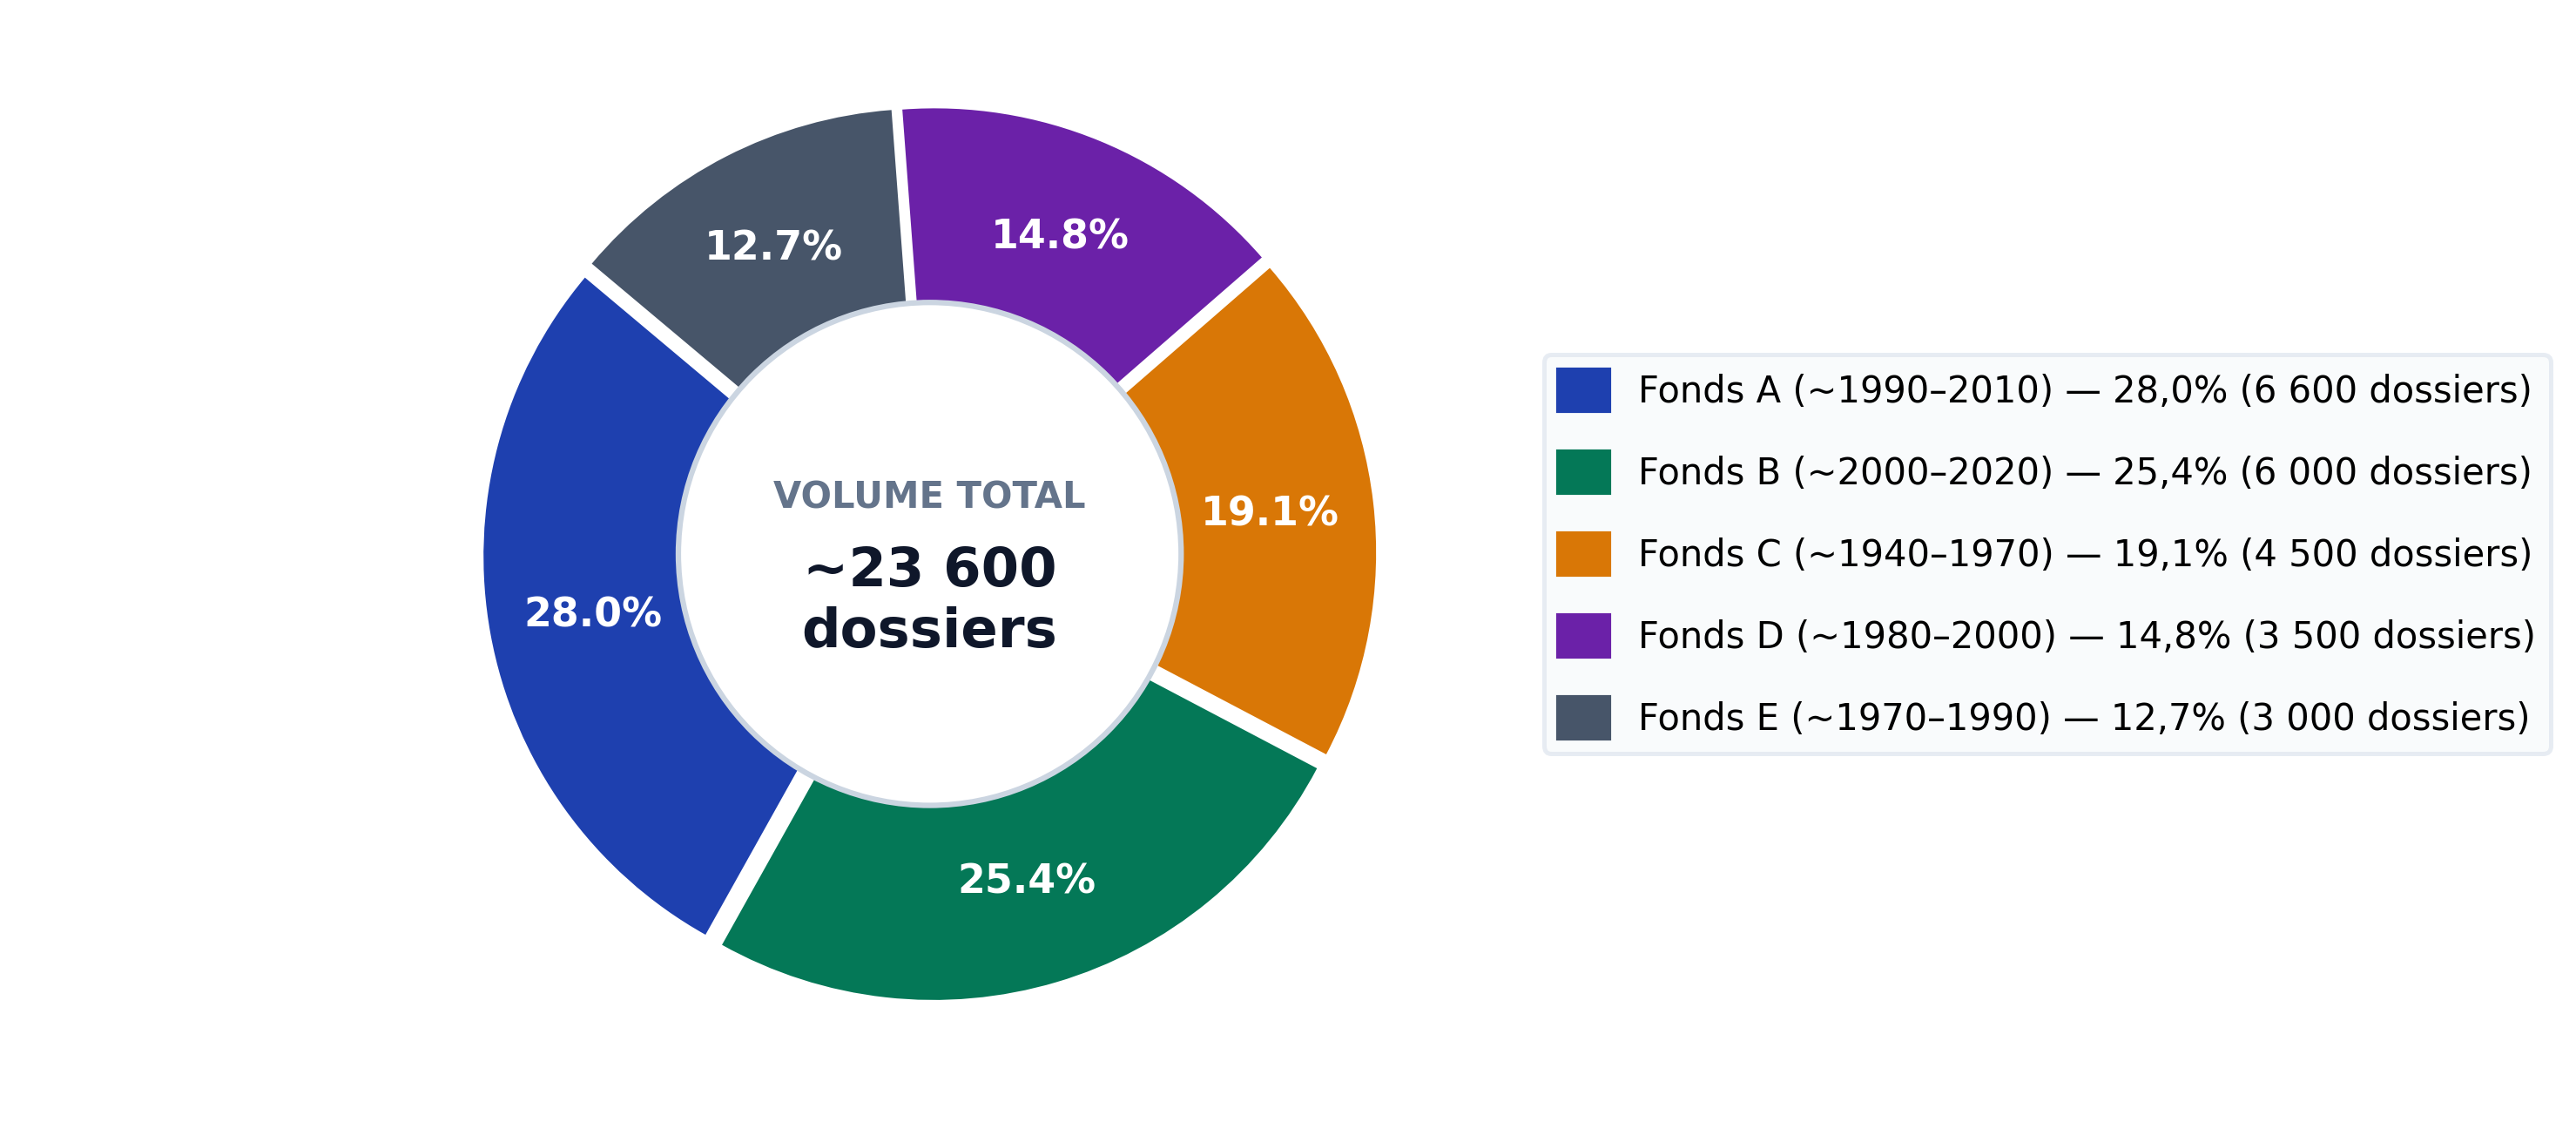
\includegraphics[width=0.95\textwidth]{img/repartition_archives.png}
  \caption{Répartition estimée du fonds d'archives du cabinet par fonds de géomètres prédécesseurs (Volume total : environ 23~600 dossiers).}
  \label{fig:repartition_archives}
\end{figure}

Chaque dossier contient l'ensemble des pièces d'une affaire : les actes fonciers (DMPC d'époque, PV et plans de bornage), les documents administratifs (devis, factures, courriers) et les notes de mesures terrain.

Pour le traitement automatique, on distingue trois grandes catégories de documents :

Les registres d'affaires tenus par chaque géomètre récapitulent la liste des dossiers. Pour les plus anciens rédigés à la main, la faible qualité du contraste et l'absence de grille fixe selon le prédécesseur rendent la lecture difficile.

Les documents dactylographiés (principalement entre 1980 et 2000) ont été créés à la machine à écrire. Le bruit présent dans le document (taches, ratures, etc.) nécessite un prétraitement pour améliorer la lisibilité.

Enfin, les dossiers contiennent de nombreuses pièces annexes (devis, factures). Le projet doit savoir trier les pages pour extraire uniquement les données des actes et des registres utiles.



La recherche d'informations au sein de ces fonds d'archives nécessite de croiser les pièces d'un même dossier. L'intérêt du traitement des registres repose sur ce recoupement des données. En effet, un document comme un DMPC ne comporte pas toutes les informations nécessaires, comme le numéro de dossier interne du cabinet. En revanche, les anciens géomètres inscrivaient sur une ligne de leur répertoire la date, le numéro d'affaire, le nom du client, la commune et les parcelles concernées parfois. La structure de cette ligne dépend toutefois du géomètre d'époque qui l'a rédigée. L'objectif est donc de faire correspondre chaque ligne du registre avec le plan ou le DMPC associé pour reconstituer le dossier complet.

\subsection{Analyse des registres et des difficultés de lecture}

Ces registres ne se présentent pas tous de la même façon : chaque géomètre avait sa propre tenue, les informations disponibles varient selon le fonds, et certains champs peuvent être absents d'un registre à l'autre. Certains traçaient des colonnes fixes, d'autres rédigeaient en texte continu ou utilisaient des imprimés différents.

Cette diversité entraîne trois difficultés principales pour le projet:

Premièrement, l'absence de grille pour certains registres rend l'alignement des colonnes variable d'un à l'autre et parfois d'une page à l'autre.

Deuxièmement, l'utilisation de guillemets de répétition (\enquote{"}), d'abréviations, ou encore de la mention \enquote{Idem} pour éviter de réécrire la commune ou la date d'une ligne sur l'autre. Le projet doit savoir conserver la valeur précédente en mémoire pour reconstituer ce type de schéma.

Troisièmement, le chevauchement de l'écriture manuscrite. Comme le montre la figure~\ref{fig:registre_ancien}, certaines lettres dépassent souvent sur les lignes du dessus ou du dessous, ce qui complique la séparation des lignes de texte par cases.

\begin{figure}[H]
  \centering
  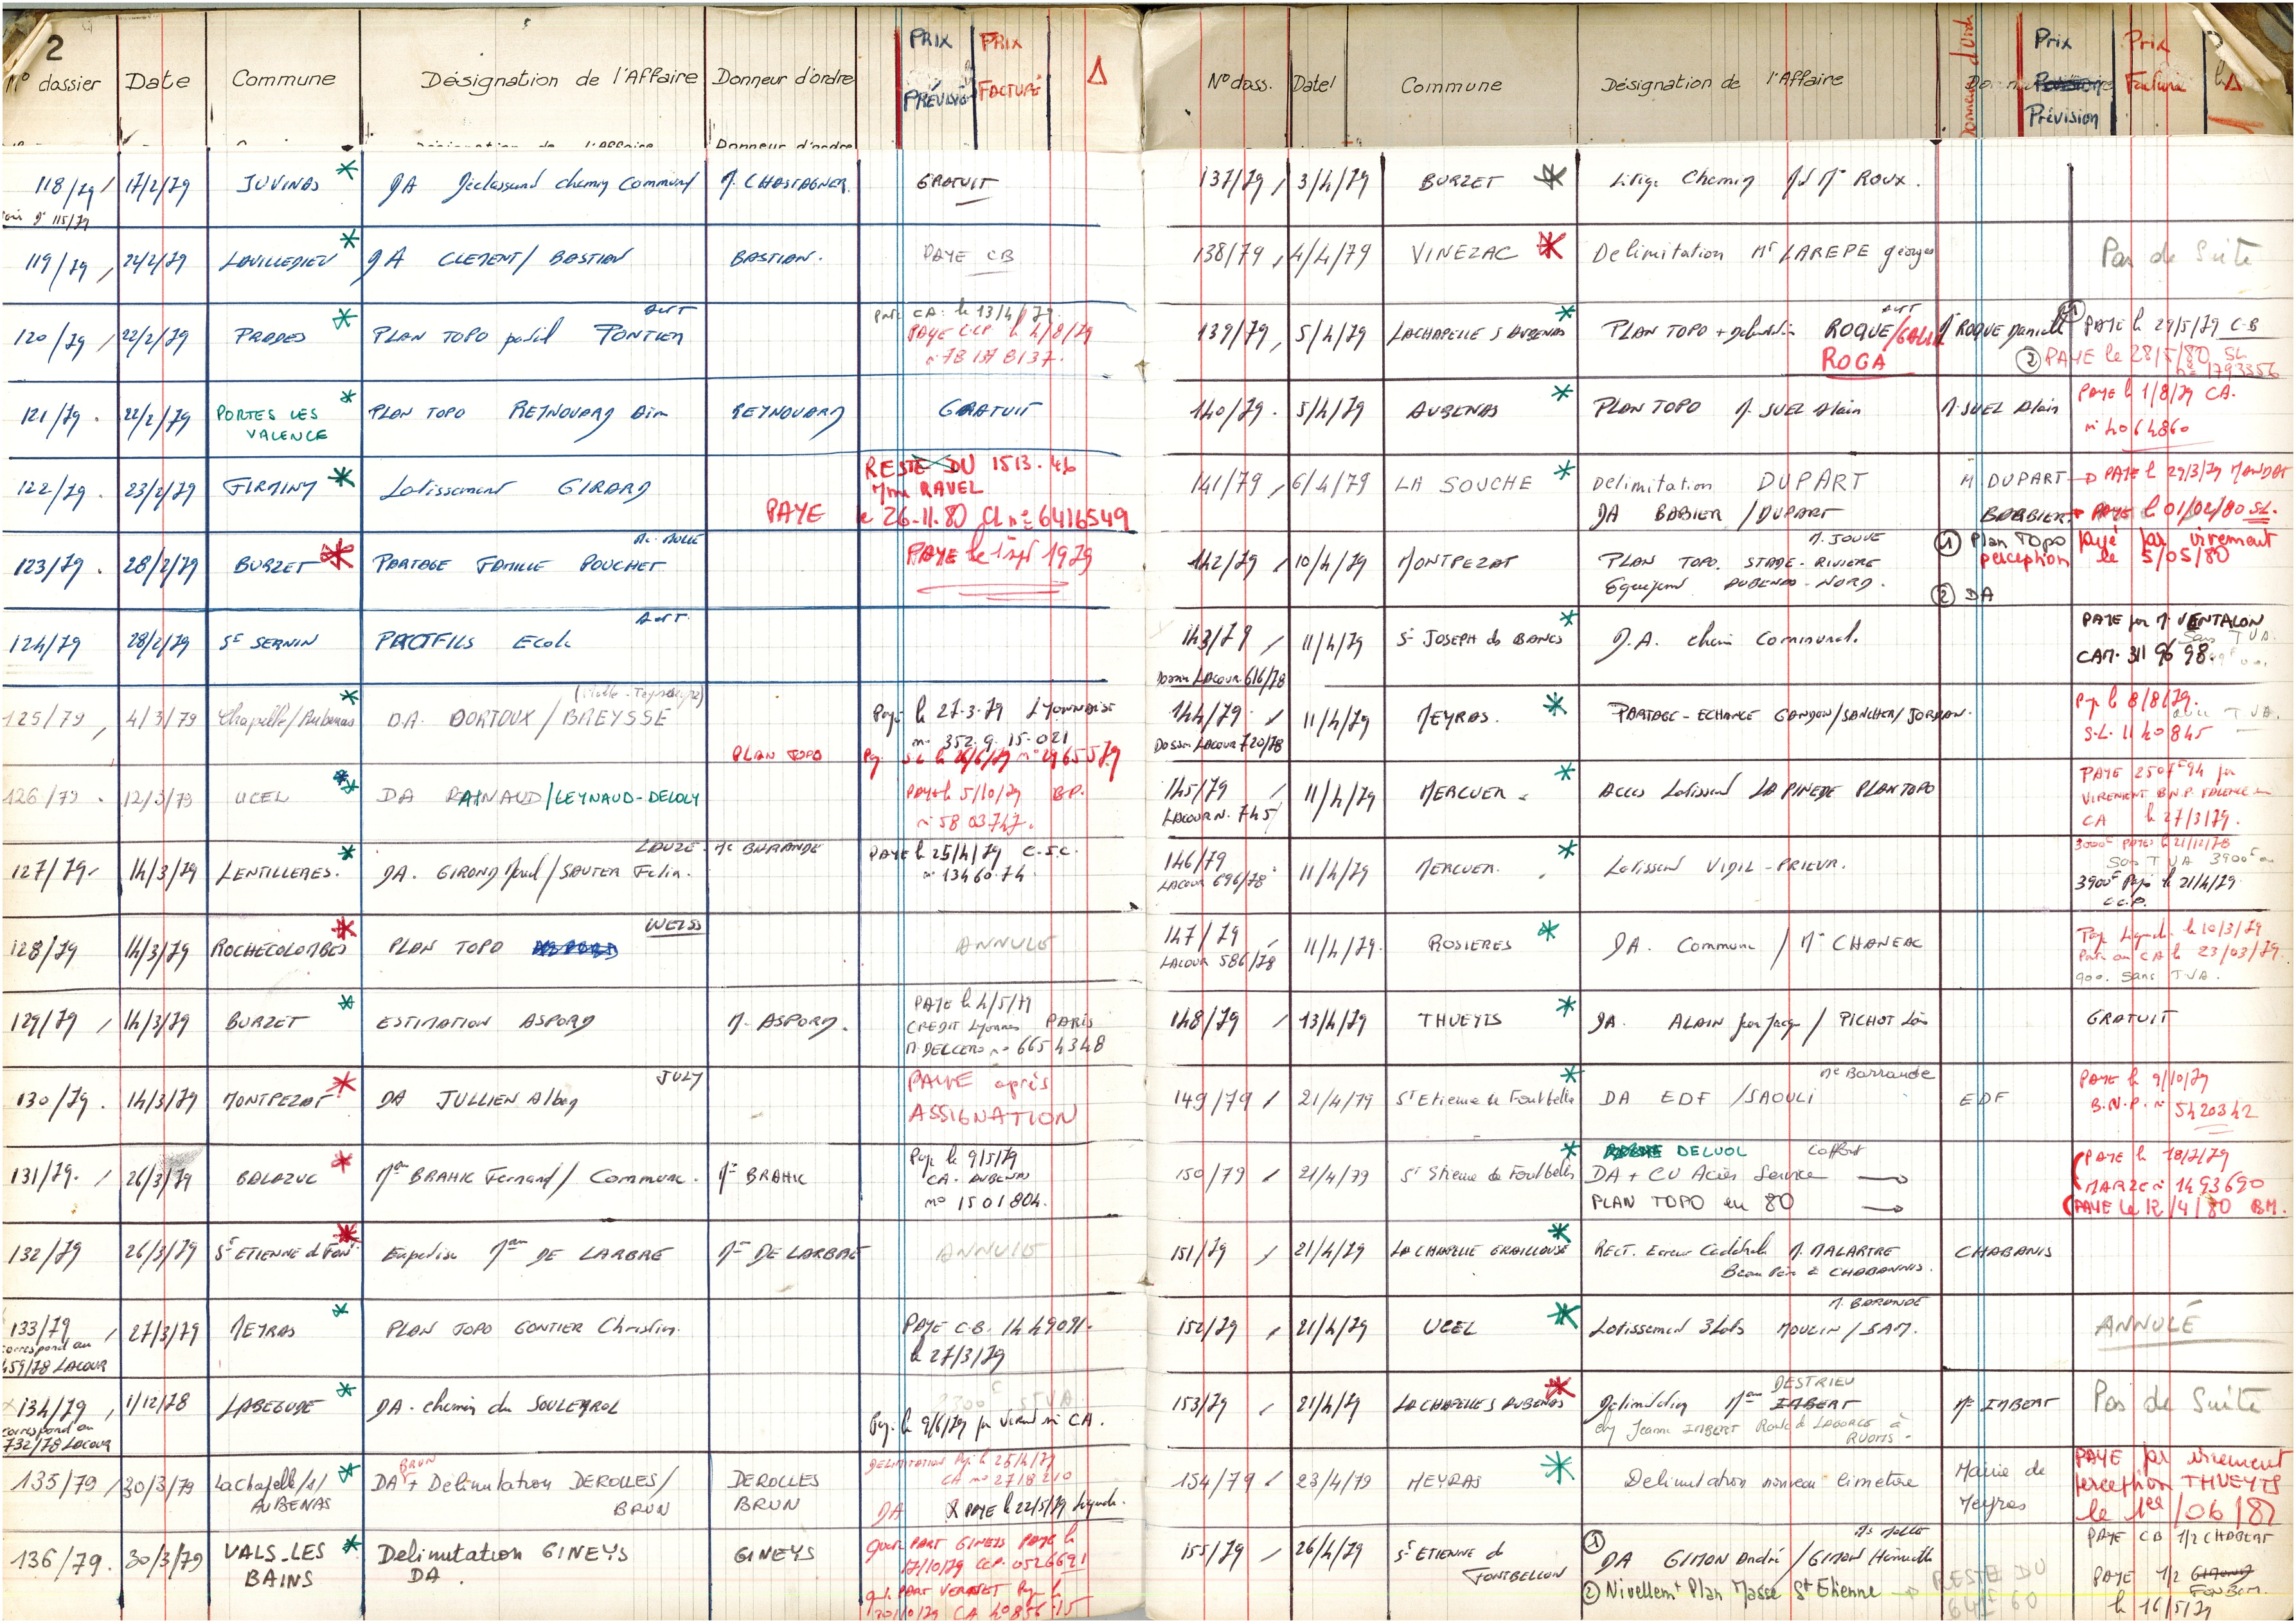
\includegraphics[width=\textwidth]{img/registre_manuscrit.jpg}
  \caption{Extrait d'un registre historique manuscrit du cabinet, illustrant l'écriture manuelle et les abréviations.}
  \label{fig:registre_ancien}
\end{figure}


La figure~\ref{fig:registre_ancien} illustre concrètement ces difficultés. On y observe deux pages d'un même registre  : la couleur de l'encre varie du noir au bleu, avec des annotations en rouge ajoutées après coup. Les colonnes sont tracées à la règle mais l'écriture déborde régulièrement d'une ligne sur l'autre. Certaines cases contiennent des abréviations, des renvois ou des symboles de répétition, tandis que d'autres sont laissées vides. La densité et le style de l'écriture changent visiblement d'un rédacteur à l'autre, parfois au sein d'une même page. On peut y distinguer les entêtes de numéro de dossier, date, commune, désignation de l'affaire, et donneur d'ordre. Ce registre couvre donc une partie des champs exigés par l'API Géofoncier : le numéro de dossier, la date et la commune sont présents. En revanche, les coordonnées géographiques de l'opération en Lambert-93 sont totalement absentes et doivent être extraites depuis le plan associé au dossier, tout comme le numéro de parcelle ainsi que de section.


Ainsi, la lecture des registres nécessite de traiter ces difficultés de présentation pour extraire correctement les données. Cependant, une fois ces informations récupérées, une autre étape est indispensable : réussir à lier les anciens numéros de parcelles aux références actuelles, qui ont pour la plupart évolué au fil des années.


\subsection{La filiation parcellaire}

La filiation parcellaire est importante pour retrouver les parcelles concernées par les archives du cabinet. Lorsqu'un géomètre recherche un dossier aujourd'hui, il dispose souvent uniquement du numéro de la parcelle actuelle. Cette même logique est à appliquer lors de la création de ces anciens dossiers. Les actes anciens ont été enregistrés sous les numéros parcellaires qui pour la plupart ont subi une modification, un découpage, ou tout autre intervention. L'un des objectif de ce projet est donc de retrouver les numéros de parcelles d'époques et de trouver une correspondance actuelle.

Lors d'une division foncière réalisée par un DMPC, l'ancien numéro de parcelle (la parcelle mère, par exemple \texttt{A 14}) est supprimé du cadastre et remplacé par de nouveaux numéros (les parcelles filles, par exemple \texttt{A 115} et \texttt{A 116}). Au fil du temps, ces nouvelles parcelles peuvent elles aussi être divisées. Sans le suivi de ces changements successifs, une recherche effectuée sur la parcelle actuelle ne permet de retrouver aucune localisation, le portail Géofoncier étant mis à jour régulièrement.

\begin{figure}[H]
  \centering
  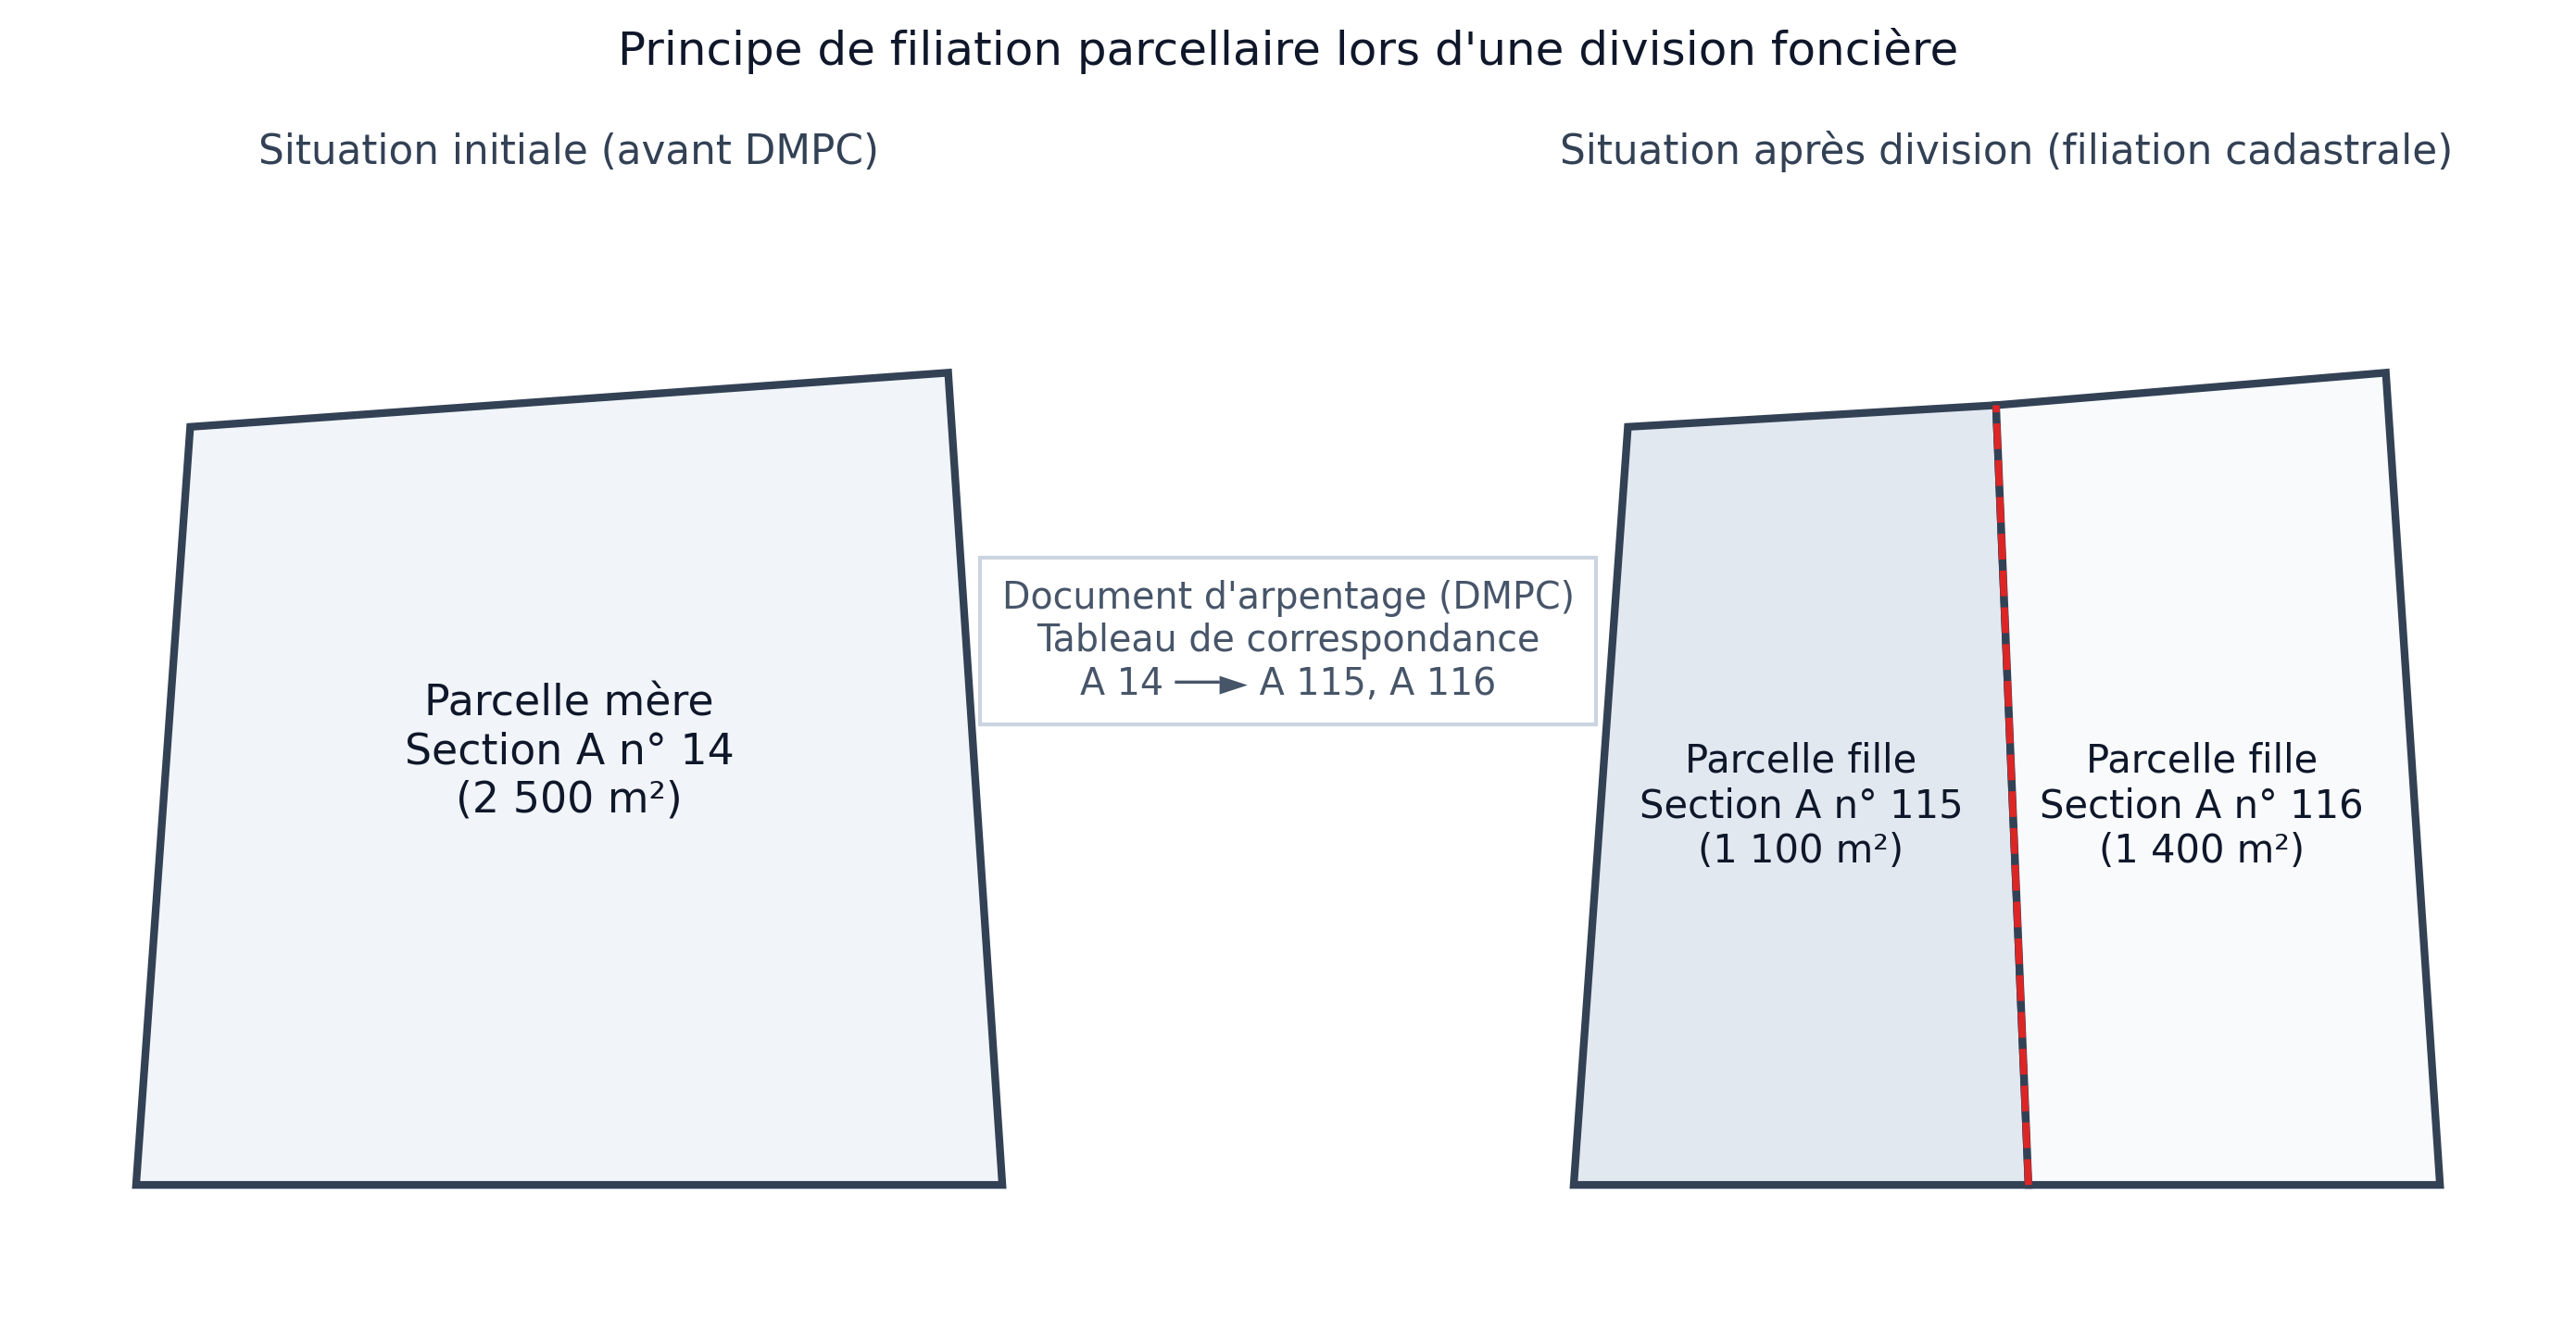
\includegraphics[width=0.95\textwidth]{img/filiation_parcellaire.png}
  \caption{Principe de filiation parcellaire lors d'un DMPC (remplacement de la parcelle mère A 14 par les parcelles filles A 115 et A 116).}
  \label{fig:filiation_parcellaire}
\end{figure}

Cette filiation est tenue à jour par la DGFiP à chaque validation d'un nouveau DMPC. Elle est enregistrée dans la matrice cadastrale et directement accessible aux géomètres sur le portail Géofoncier ainsi que par son API. Concrètement, cette base conserve l'historique des modifications sous forme d'associations entre chaque parcelle supprimée (la mère) et les parcelles créées (les filles).

En interrogeant cette base de filiation, le projet peut remonter automatiquement la chaîne des parcelles mères successives. Cela permet d'associer une parcelle contemporaine recherchée par le géomètre au numéro d'origine inscrit dans l'acte d'époque, et ainsi de retrouver le dossier correspondant. Pour ce projet, la base de données est téléchargeable sur le site de la DGFiP, et découpé par département. seul les modifications pour le département de l'Ardèche a été retenu. 


\subsection{Les contraintes de numérisation}

La réussite de l'extraction automatique dépend directement de la qualité des documents papier et des choix faits lors de leur numérisation au cabinet. Les archives conservées présentent en effet plusieurs types de détériorations physiques.

Avec le temps, le papier et les calques vieillissent et jaunissent, ce qui réduit le contraste entre l'encre et le fond. Sur les calques transparents, l'écriture du verso transparaît souvent au scanner et se mélange au texte du recto. De plus, la manipulation des dossiers au fil des années a laissé des plis et des déchirures. Il n'est pas rare non plus de trouver des annotations ajoutées après coup au crayon ou au stylo par les géomètres, qui viennent surcharger le document d'origine.

Sur les DMPC en particulier, les tampons officiels de réception posés par le cadastre (souvent avec une encre rouge ou bleue) recouvrent fréquemment le cartouche et masquent une partie des numéros de parcelles.

Toutes ces contraintes imposent de régler soigneusement les paramètres de numérisation selon le type de pièce, afin de conserver la meilleure lisibilité possible (tableau~\ref{tab:param_numerisation}).


\begin{table}[H]
  \centering
  \caption{Paramètres de numérisation retenus selon la nature des pièces d'archives.}
  \label{tab:param_numerisation}
  \small
  \begin{tabular}{p{4.5cm} c c c}
    \toprule
    \textbf{Type de document} & \textbf{Résolution (DPI)} & \textbf{Mode couleur} & \textbf{Format de fichier} \\
    \midrule
    Registres manuscrits  & 300 DPI & Niveaux de gris & PDF / TIFF  \\
    Formulaires DMPC et DA & 300 DPI & Couleur (24 bits) & PDF  \\
    PV de bornage et actes & 300 DPI & Niveaux de gris & PDF  \\
    Plans grand format (A3/A2) & 200 DPI & Couleur (24 bits) & PDF / JPEG \\
    Pièces annexes (factures) & 200 DPI & Noir et blanc & PDF  \\
    \bottomrule
  \end{tabular}
\end{table}

Le mode couleur est indispensable pour les formulaires comportant des tampons ou des traits de couleur, car il permet aux algorithmes de prétraitement de séparer les tampons de l'encre du texte, ou alors de comprendre quelles sont les anciennes ou les nouvelles parcelles.



\subsection{Synthèse des contraintes et des besoins du projet}


À la suite de cette analyse du métier, des archives et du fonctionnement de l'API, plusieurs contraintes et besoins ressortent pour le projet :

Tout d'abord, la conformité des données pour l'API exige de transmettre une structure JSON exacte respectant les formats attendus (code INSEE à 5 chiffres, date ISO 8601 et coordonnées en Lambert-93).

Ensuite, le tri des documents et le recoupement des informations imposent d'isoler les actes utiles (DMPC, PV de bornage) des pièces annexes (devis, factures) et de croiser les données des registres avec les pièces scannées pour compléter les informations manquantes.

De plus, la recherche par la filiation parcellaire doit s'appuyer sur l'historique des parcelles pour faire le lien entre les numéros d'époque figurant sur les archives et les numéros actuels recherchés.

Enfin, la confidentialité et l'exécution locale imposent que l'ensemble des traitements d'analyse d'image et d'extraction de texte s'effectue directement sur les postes du cabinet, sans envoyer de données sur des serveurs externes.

Ainsi, ces différentes exigences imposent de s'appuyer sur des solutions techniques capables de traiter aussi bien des documents imprimés que des registres manuscrits. Le chapitre suivant présente l'état de l'art des technologies d'extraction et d'analyse documentaire afin de sélectionner les outils les plus adaptés aux besoins du cabinet.
